\section{Flow Steering and Processing Allocation Problem}

%%%%%%%%%%%%%%%%%%%
%%%%%%%%%%%
%Basic problem
%%%%%%%%%%%
%%%%%%%%%%%%%%%%%%
\subsection{The basic problem}
We first solve the routing and steering problem for the above graph model: given all edge capacities $B(e)$ and vertex capacities $C(v)$ and a flow demand pattern $\mathbf{D}$, the optimization problem asks for a routing pattern with minimum congestion, the congestion can be interpreted in utilization. Like Max-flow model, we have capacitated edge constraints. However, our graph model has an extra constraint: vertex processing capacities, and it throttles the flow in a different manner: since a single flow is divisible and can be handled at different vertices, the flow is not constrained by a single node's processing power, but depending on all the nodes in the path(s). So a feasible flow pattern satisfies: (i) the edge capacities, (ii) the vertex capacities, and (iii) the relations between flow demand and processing demand. Without loss of generality, we assume the flow demand equals processing demand. 

Path-based formulation is built directly on the definition of the problem, and it takes paths as abstractions. We can also formulate an edge-based linear programming model. We can prove that they are equivalent(Proof see appendix). 

Notations: $f(U)$ is a convex function with a high penalty for high utilization. $B(e), C(v)$ are edge and vertex capacities, $D_i$ is the demand for flow i. For path-based formulation, $p(\pi,e)$ represents the processing work done at $v$ where $e\equiv(u,v)$, and $P_i$ is a set of path for flow i with $D_i$. For edge-based solution, $p_i(v)$ is the processing work done at v for flow $i$, and $w_i(e)$ is the process work demand at edge $e$ for flow $i$. 
Utilizations for edge and vertex are:
$U(e) = \frac{\sum\limits_i\sum \limits_{\pi\in P_i:e\in \pi} f(\pi)}{B(e)}=\frac{\sum\limits_{i} f_{i}(e)} {B(e)}$ and 
$U(v) = \frac{ \sum\limits_i \sum \limits_{\pi\in P_i} \sum \limits_{ e\in \pi} p(\pi, e) } {C(v)}=\frac{ \sum\limits_i p_i(v)}{C(v)}$.

\begin{minipage}[t]{0.45\textwidth}
\textit{Path-based formulation:}
  \begin{subequations}
\begin{align}
\text{Minimize:} & \sum \limits_{e} f(U(e)) + \sum \limits_{v} f(U(v)) \\  \nonumber
\text{Subject } &\text{to:} \\
\forall i,& \forall \pi\in P_i; \sum \limits_{e\in \pi} p(\pi, e) = f(\pi)\\
\forall i;& \sum\limits_{\pi\in P_i}f(\pi) = D_i\\
\forall \pi,&\forall e;p(\pi,e) \geq 0
\end{align}
\end{subequations}
  \end{minipage}
\hspace{0cm}
\begin{minipage}[t]{0.50\textwidth}
\textit{Edge-based formulation:}
  \begin{subequations}
\begin{align}
\text{Minimize:}&\sum \limits_{e} f(U(e)) + \sum \limits_{v} f(U(v)) \\ \nonumber
\text{Subject } &\text{to:}\\
\forall v \not= s,t,\forall i;& \sum\limits_{in}  f_i(e)=  \sum\limits_{out} f_i(e)\\
\forall v,\forall  i; p_i(v)& = \sum\limits_{in} w_i(e) - \sum\limits_{out} w_i(e) \\
\forall  i, \forall (s-v); &\sum\limits_v f_i(e)= D_i\\
\forall  i,\forall (s-v);& w_i(e)= f_i(e)\\
\forall  i,\forall (v-t);& w_i(e)= 0\\
\forall e,\forall i;w_i(e),& f_i(e)-w_i(e), p_i(v) \geq 0
\end{align}
\end{subequations}
\end{minipage}

Understand edge-based formulation: 2.2b is the same flow conservation, and 2.2c, g $p_i(v)$ shows the flow demand should be decreasing, 2.2d, e, f ensures the flow demand and process demand relations. 

%%%%%%%%%%%%%%%%%%%
%%%%%%%%%%%
%Flow size change
%%%%%%%%%%%
%%%%%%%%%%%%%%%%%%
\emph{Flow Size Changes after Processing:} the basic model shows that in-network processing does not affect the traffic size. However the change of flow size after processing is a common case in networking, for example, encryption increases the flow size while compression and transcoding decrease the traffic size\cite{Mogul1997}. We can capture this aspect and integrate into the optimization formulation. In generalized minimum cost circulation problem \cite{Wayne1999}, there is a gaining factor. We apply the same idea, but one key difference in our model is that flow size change only applies the gaining factor to part of the flow to be processed at the vertex. 

The change can be easily captured in the formulation, if there is a size change, at each vertex, we have $\sum\limits_{in} w(e) - \sum\limits_{out}  w(e) = p(v)$ and $\sum\limits_{out} (f(e) - w(e))-\sum\limits_{in}  (f(e) - w(e))= p(v)*r$, assume $r$ is a positive gaining factor. If $r=1$, we have exactly the flow conservation $\sum\limits_{out} f(e) -\sum\limits_{in}  f(e)= 0$. 

%%%%%%%%%%%%%%%%%%%
%%%%%%%%%%%
%Mutiple tasks as a DAG
%%%%%%%%%%%
%%%%%%%%%%%%%%%%%%

\subsection{Multiple tasks as a DAG}
In practice, a flow usually needs several different processes before sink. In the above formulation we assume there is only one task, or each vertex can run all types of flow processing where we can bundle all tasks into one task. Nevertheless if we have specialized hardware or two types of processing are preferred to be separated at different vertices, we need to revisit our formulation. 
We consider two common types of task relationships: serial and parallel. Serial tasks must be handled in a certain order while parallel tasks can happen in any order. We can satisfy the new requirement by modifying the optimization formulation. We consider two corner cases where there are N serial or N parallel tasks, and then we extend this to a general case where N tasks have a DAG relation. 

For $N$ serial tasks, we have $C^n(v); n\in\{1\dots N\}$ for $N$ different processing capacities. In optimization formulation 2.2, we can think of two different types of flows, pre-processed and post-processed, and in this model we have $N+1$ types of flows: pre-$n$-post-$(n-1)$ processed where $ n\in\{1\dots N\}$ and  fully processed flows. We can extend formulation 2.2 by adding $N-1$ process demands, in particular for 2.2c we extend to N different types of processing, $p_i^n= \sum\limits_{in} w_i^n(e) - \sum\limits_{out} w_i^n(e)$. Besides the same capacity and flow relation constraints, we also need $w_i^n(e) \geq w_i^{n-1}(e)$ where it reflects the sequence. The complexity of this formulation increases in a linear relation to the number of tasks $N$.
\begin{figure}
 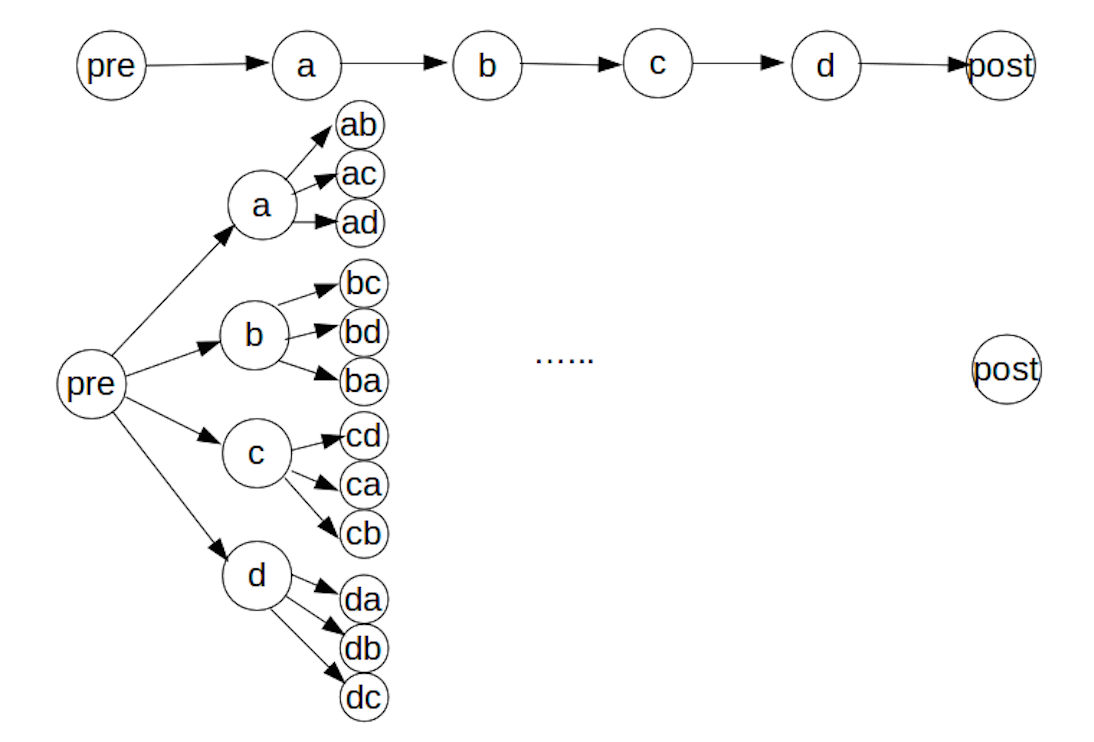
\includegraphics[width=\linewidth]{task.png}
 \caption{Up: serial tasks, Down: parallel tasks; a,b,c represents three different tasks and each link represents one dependency}
\end{figure}


For $N$ parallel tasks, again we have $C^n(v); n\in\{1\dots N\}$ for $N$ different processing capacities. Unlike serial relation, the number of types of flow grows exponentially, at most there can be $2^N$ types of flows. We have $O(2^N)$ inequalities represents the dependencies and $O(N)$ inequalities represents processing capacity relations.
% Surprisingly the complexity of the formulation also increases in a linear relation to the number of tasks N if we utilize the independence between tasks. The constraints are almost the same as above serial case except for that there is no sequential constraint like $w_i^n(e) \geq w_i^{n-1}(e)$. This optimization problem is similar to solve $N$ separate optimization problems and the $N$ problems are linked by the routing choice $f_i$ and the objective function. We argue that the optimization solution also provides with enough information for routing and processing decision; we can process the flow in the following manner: each flow has $N$ tags which indicates whether the part of the flow $n\in\{1\dots N\}$ is processed, and since the order can be arbitrary for $N$ processings, for each type of processing, it only needs to check its corresponding tag and make decisions independently. 

To generalize, if there are tasks with a DAG relation where each directed link $(p,q)$ represents a dependency of $q$ to $p$, there is an inequality relation $w_i^q(e) \geq w_i^p(e)$ for each link $(p,q)$. For any k parallel tasks, we need to build $O(2^k)$ branches and establish the relation using the method above.   
